\documentclass[conference]{IEEEtran}
\IEEEoverridecommandlockouts

% Engine-aware font and encoding setup (reproducible TeX Gyre Times metrics under XeTeX/Tectonic)
\usepackage{iftex}
\ifXeTeX
  \usepackage{fontspec}
  \setmainfont{texgyretermes-regular.otf}[
    BoldFont = texgyretermes-bold.otf,
    ItalicFont = texgyretermes-italic.otf,
    BoldItalicFont = texgyretermes-bolditalic.otf
  ]
  \setsansfont{texgyreheros-regular.otf}[
    BoldFont = texgyreheros-bold.otf,
    ItalicFont = texgyreheros-italic.otf,
    BoldItalicFont = texgyreheros-bolditalic.otf
  ]
  \setmonofont[Scale=0.86]{texgyrecursor-regular.otf}[
    BoldFont = texgyrecursor-bold.otf
  ]
\else
  \usepackage[T1]{fontenc}
  \usepackage[utf8]{inputenc}
\fi

% Packages
\usepackage{cite}
\usepackage{amsmath,amssymb,amsfonts}
\usepackage{graphicx}
\usepackage{textcomp}
\usepackage{xcolor}
\usepackage{listings}
\usepackage[hyphens]{url}
\usepackage{booktabs}
\usepackage{array}
\usepackage{tikz}
\usetikzlibrary{shapes.geometric,arrows.meta,positioning,calc,fit,backgrounds,decorations.pathreplacing}
\usepackage{hyperref}
\def\UrlBreaks{\do\/\do-\do_\do.\do=\do?\do&}

\hypersetup{
    colorlinks=true,
    linkcolor=black,
    citecolor=black,
    urlcolor=blue
}

% Code listing configuration
\lstset{
    basicstyle=\ttfamily\footnotesize,
    breaklines=true,
    captionpos=b,
    numbers=left,
    numberstyle=\tiny\color{gray},
    keywordstyle=\color{blue}\bfseries,
    commentstyle=\color{olive}\itshape,
    stringstyle=\color{red},
    showstringspaces=false,
    tabsize=2
}

\def\BibTeX{{\rm B\kern-.05em{\sc i\kern-.025em b}\kern-.08em
    T\kern-.1667em\lower.7ex\hbox{E}\kern-.125emX}}

\begin{document}

\title{Blind Cognitive Multi-Factor Authentication Architecture for Untrusted Web and Mobile Endpoints under OpenID Connect\thanks{Research proposal and short scientific paper developed for the course \textit{Web and Mobile Systems Security}, Master of Science in Cybersecurity and Computer Systems Auditing, Polytechnic Institute of Gaya (ISPGAYA), Academic Year 2026/2027.}}

\author{\IEEEauthorblockN{Carlos Andr\'e Sousa}
\IEEEauthorblockA{\textit{M.Sc. in Cybersecurity and Computer Systems Auditing} \\
\textit{Polytechnic Institute of Gaya (ISPGAYA)}\\
Vila Nova de Gaia, Portugal \\
Student No. 2022105675 \\
casousa@ispgaya.pt}
}


\maketitle

% Core structured sections
\begin{abstract}
Traditional Multi-Factor Authentication (MFA) mechanisms fail when the client endpoint is untrusted or compromised by infostealer malware, screen grabbers, or adversary-in-the-middle proxies. While hardware-bound tokens (FIDO2/WebAuthn) protect against network relay, they remain vulnerable to malware-induced session hijacking post-authentication and face physical availability constraints in ad-hoc web and mobile environments. This paper proposes a Blind Cognitive Multi-Factor Authentication (BC-MFA) architecture designed for untrusted web and mobile public clients. The protocol decouples the visual display on the terminal from the user's authentic credential computation through dynamic, quadrant-balanced toroidal challenge-response matrices, paired with passive behavioral anomaly detection (cognitive hesitation, pointer/touch kinematics, and keystroke cadence). We formalize the protocol exchange under OpenID Connect (OIDC) Core 1.0 and OAuth 2.0, combining RFC 7636 PKCE, registered RFC 8176 Authentication Method Reference (\texttt{amr}) claims, and RFC 9449 Demonstrating Proof-of-Possession (DPoP) access token binding. Analytical threat modeling and a reproducible 500-trial Monte Carlo intersection simulation quantify resilience against keyloggers, screen scrapers, SIM swapping, multi-session intersection attacks, and automated relay bots without requiring dedicated client cryptographic hardware, while explicitly scoping first-contact active reverse-proxy limits. Finally, we establish a literature-grounded latency model and the formal empirical evaluation plan for the Master's dissertation.
\end{abstract}

\begin{IEEEkeywords}
\normalfont
Cognitive authentication, untrusted endpoints, infostealers, OpenID Connect, RFC 8176, RFC 9449, behavioral anomaly detection, challenge-response.
\end{IEEEkeywords}

\section{Introduction}
\label{sec:introduction}

Client endpoints represent the most vulnerable perimeter in modern web and mobile application security~\cite{syed2022zero}. While identity providers (IdPs) enforce robust server-side cryptography, user interactions terminate on client devices that frequently operate outside corporate control~\cite{jannett2024sok}. Bring Your Own Device (BYOD) policies, shared public workstations, and commodity operating systems expose users to host-level threats, including credential-harvesting malware, memory scrapers, and malicious browser extensions~\cite{gautam2025passwords, lee2024beneath}. In this threat environment, traditional authentication factors fail. Passwords and one-time codes transmitted across compromised input devices are recorded instantly by low-level keyloggers~\cite{amft2023weve}.

To counter phishing and network relay, industry standards have converged on hardware-anchored credentials, specifically FIDO2/WebAuthn~\cite{angelogianni2024how, nist80063b4}. WebAuthn deterministically halts network-level Adversary-in-the-Middle (AitM) proxies through public-key cryptography bound to the browser origin~\cite{golaszewski2026binding}. However, WebAuthn assumes an uncompromised client operating environment. When malware or reverse-proxy toolkits target the session lifecycle, adversaries intercept bearer session tokens post-authentication or exploit UI overlay deception on client devices~\cite{mahdad2024breaching, hilbig2023protect, lim2025phishers}. Furthermore, hardware security keys face physical distribution, recovery, and user adoption barriers in consumer web applications and public terminal settings~\cite{kepkowski2023challenges}.

This paper proposes the \textit{Blind Cognitive Multi-Factor Authentication} (BC-MFA) architecture. BC-MFA addresses step-up authentication on untrusted web and mobile endpoints without requiring external cryptographic hardware tokens. The core mechanism separates the visual stimuli displayed on the untrusted screen from the actual secret verified by the IdP. The server issues a dynamic cognitive challenge: an ephemeral, quadrant-balanced visual transformation matrix. The user mentally combines the challenge with a pre-shared cognitive secret (a private anchor quadrant and a non-zero toroidal geometric offset path) to generate a one-time response~\cite{binbeshr2025challenge}. An adversary capturing keystrokes or recording the display learns neither the underlying secret nor the rule governing subsequent challenges. To mitigate automated bot replay and remote human solver delegation, BC-MFA couples this cognitive ceremony with passive behavioral anomaly telemetry capturing cognitive hesitation latency, pointer or touchscreen kinematics, and keystroke cadence~\cite{incel2021dakota, khan2024mouse}.

Three concrete research questions guide this inquiry. First, \textbf{RQ1} examines whether quadrant-balanced challenge-response permutations over toroidal grids can guarantee bounded combinatorial ambiguity against continuous display capture across $k$ compromised sessions while keeping expected human mental latency within practical bounds ($\le 5\text{ s}$). Second, \textbf{RQ2} investigates the protocol bindings required to integrate cognitive verification, RFC 7636 PKCE, and RFC 9449 Demonstrating Proof-of-Possession (DPoP) access token binding into standard OpenID Connect Core 1.0 public-client flows using registered RFC 8176 Authentication Method Reference (\texttt{amr}) claims without requiring mandatory relying party modifications. Third, \textbf{RQ3} evaluates whether passive interaction kinematics (cognitive hesitation, pointer/touch trajectories, and short-input keystroke cadence) provide sufficient discriminatory signal to separate authentic human operators from automated replay bots and off-device relay solvers on heterogeneous endpoints.

This paper delivers four core contributions. First, it defines the formal protocol specification and worked toroidal transformation mechanics for Blind Cognitive MFA on untrusted web and mobile public clients. Second, it specifies a standards-compliant federation profile mapping cognitive, behavioral, PKCE, and DPoP key-binding ceremonies into OpenID Connect Core 1.0 using RFC 7636, RFC 8176, and RFC 9449. Third, it provides a mathematical threat evaluation (covering keyloggers, screen scrapers, SIM swapping, and AitM proxies, while demarcating first-contact active reverse-proxy limits) validated by a reproducible 500-trial rational-adversary Monte Carlo intersection simulation. Fourth, it establishes a literature-grounded latency model and a formal, ethics-compliant empirical evaluation plan for the Master's dissertation.

Section~\ref{sec:methodology_and_prisma} details the systematic literature review methodology. Section~\ref{sec:related_work} positions this proposal relative to existing cognitive and biometric literature. Section~\ref{sec:architecture} details the system architecture, worked toroidal matrix transformations, and OpenID Connect token bindings. Section~\ref{sec:security_analysis} provides formal threat modeling and Monte Carlo intersection analysis. Section~\ref{sec:usability_and_overhead} analyzes cognitive latency bounds, fault tolerance, and accessibility. Section~\ref{sec:experimental_design_and_thesis} formalizes the empirical dissertation evaluation framework, and Section~\ref{sec:conclusion} concludes the paper.

\section{Systematic Literature Review Methodology (PRISMA 2020)}
\label{sec:methodology_and_prisma}

\subsection{Review Protocol and Scoped Retrieval Strategy}
To establish an evidence-grounded baseline for cognitive authentication on untrusted web and mobile endpoints, this study executes a systematic literature review following the PRISMA 2020 reporting guideline~\cite{page2021prisma} and domain-specific phishing review protocols~\cite{naqvi2023mitigation}. We queried four primary scientific databases: the ACM Digital Library, IEEE Xplore, ScienceDirect (Elsevier), and SpringerLink. To maintain tractability and avoid broad single-facet noise, retrieval enforced a three-way conjunction across title and author-keyword metadata, restricting results to peer-reviewed security and human-computer interaction venues published between January 2021 and October 2026:

\begin{quote}\raggedright\footnotesize\ttfamily
("authentication" OR "multi-factor" OR "FIDO2" OR "OpenID Connect" OR "OAuth 2.0") AND ("untrusted" OR "phishing" OR "adversary-in-the-middle" OR "infostealer" OR "shoulder surfing") AND ("cognitive" OR "challenge-response" OR "behavioral biometrics" OR "keystroke dynamics" OR "mouse dynamics" OR "token binding" OR "session hijacking")
\end{quote}

In accordance with PRISMA 2020 dual-channel identification, foundational protocol standards were identified separately via normative standards bodies (IETF, OpenID Foundation, NIST, and W3C)~\cite{oidc_core1, nist80063b4, rfc6238totp, rfc6749oauth, rfc7636pkce, rfc8176amr, rfc9449dpop, rfc9700bcp, w3cwebauthn3}, including pre-2021 RFCs retained as active normative baselines.

\subsection{Eligibility Criteria and PRISMA Selection Workflow}
Database records underwent formal evaluation against predefined eligibility criteria. Inclusion required: (1) archival publication in peer-reviewed journals or conference proceedings with verifiable Digital Object Identifiers (DOIs), (2) reproducible formal security proofs, protocol measurements, or empirical human usability data, and (3) direct applicability to web or mobile authentication environments. Exclusion removed duplicates, off-topic titles/abstracts, non-archival short posters or editorial summaries, legacy desktop-only smartcard architectures, and papers lacking quantitative security or usability evaluation. Figure~\ref{fig:prisma_tp2} presents the dual-channel PRISMA 2020 selection workflow.

\begin{figure}[!t]
\centering
\resizebox{\columnwidth}{!}{%
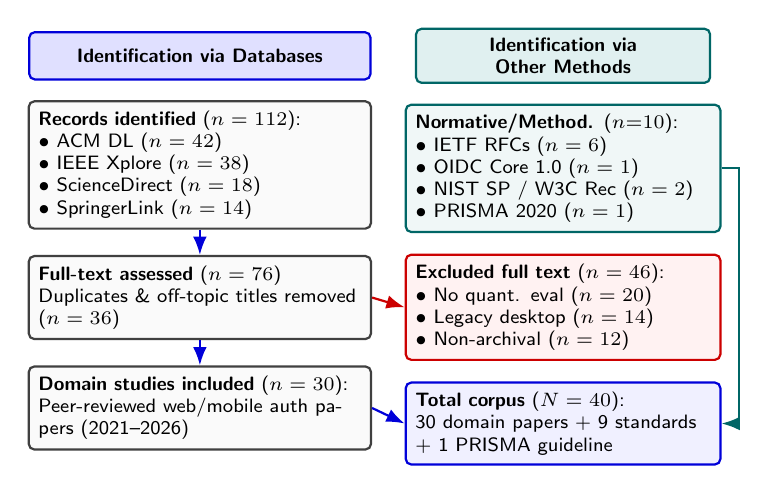
\begin{tikzpicture}[
    font=\sffamily\scriptsize,
    hdr/.style={rectangle, draw=blue!85!black, fill=blue!12, thick, rounded corners=2pt, align=center, font=\sffamily\bfseries\scriptsize, minimum height=0.6cm},
    box/.style={rectangle, draw=black!75, fill=gray!4, thick, rounded corners=2pt, align=left, font=\sffamily\scriptsize\raggedright, inner sep=3.5pt},
    exclbox/.style={rectangle, draw=red!80!black, fill=red!5, thick, rounded corners=2pt, align=left, font=\sffamily\scriptsize\raggedright, inner sep=3.5pt},
    normbox/.style={rectangle, draw=teal!80!black, fill=teal!6, thick, rounded corners=2pt, align=left, font=\sffamily\scriptsize\raggedright, inner sep=3.5pt},
    arrow/.style={-Latex, thick, draw=blue!85!black},
    sidearrow/.style={-Latex, thick, draw=red!80!black},
    normarrow/.style={-Latex, thick, draw=teal!80!black}
]
    % Column Headers
    \node[hdr, text width=4.1cm] (h_db) {Identification via Databases};
    \node[hdr, draw=teal!80!black, fill=teal!12, text width=3.5cm, right=0.55cm of h_db] (h_oth) {Identification via Other Methods};

    % Left Branch: Databases
    \node[box, text width=4.1cm, below=0.25cm of h_db] (db_ident) {
        \textbf{Records identified} ($n = 112$):\\
        $\bullet$ ACM DL ($n = 42$)\\
        $\bullet$ IEEE Xplore ($n = 38$)\\
        $\bullet$ ScienceDirect ($n = 18$)\\
        $\bullet$ SpringerLink ($n = 14$)
    };

    \node[box, text width=4.1cm, below=0.32cm of db_ident] (db_screen) {
        \textbf{Full-text assessed} ($n = 76$)\\
        Duplicates \& off-topic titles removed ($n = 36$)
    };

    \node[box, text width=4.1cm, below=0.32cm of db_screen] (db_incl) {
        \textbf{Domain studies included} ($n = 30$):\\
        Peer-reviewed web/mobile auth papers (2021--2026)
    };

    % Right Branch: Exclusions + Normative Standards
    \node[normbox, text width=3.75cm, below=0.25cm of h_oth] (oth_norm) {
        \textbf{Normative/Method.} ($n{=}10$):\\
        $\bullet$ IETF RFCs ($n = 6$)\\
        $\bullet$ OIDC Core 1.0 ($n = 1$)\\
        $\bullet$ NIST SP / W3C Rec ($n = 2$)\\
        $\bullet$ PRISMA 2020 ($n = 1$)
    };

    \node[exclbox, text width=3.75cm, below=0.26cm of oth_norm] (db_excl) {
        \textbf{Excluded full text} ($n = 46$):\\
        $\bullet$ No quant. eval ($n = 20$)\\
        $\bullet$ Legacy desktop ($n = 14$)\\
        $\bullet$ Non-archival ($n = 12$)
    };

    \node[normbox, draw=blue!85!black, fill=blue!6, text width=3.75cm, below=0.26cm of db_excl] (tot_incl) {
        \textbf{Total corpus} ($N = 40$):\\
        30 domain papers + 9 standards + 1 PRISMA guideline
    };

    % Connectors
    \draw[arrow] (db_ident.south) -- (db_screen.north);
    \draw[arrow] (db_screen.south) -- (db_incl.north);
    \draw[sidearrow] (db_screen.east) -- (db_excl.west);
    \draw[arrow] (db_incl.east) -- (tot_incl.west);
    \draw[normarrow] (oth_norm.east) -- ++(0.22,0) |- (tot_incl.east);
\end{tikzpicture}%
}
\caption{Dual-channel systematic literature and normative selection workflow adapted from PRISMA 2020.}
\label{fig:prisma_tp2}
\end{figure}

Scoped title-and-keyword querying retrieved $n = 112$ initial database records. Removing duplicates and off-topic titles excluded $n = 36$ entries, leaving $n = 76$ full-text candidates. Full-text eligibility screening excluded $n = 46$ records: 20 lacked quantitative usability or security evaluation, 14 relied on legacy desktop-only smartcard dependencies, and 12 were non-archival posters or out-of-scope summaries, yielding exactly $n = 30$ peer-reviewed domain studies ($76 - 46 = 30$). Via the separate normative channel, we incorporated 9 formal protocol specifications (6 IETF RFCs, OpenID Connect Core 1.0, NIST SP 800-63B-4, and W3C WebAuthn Level 3) alongside the PRISMA 2020 reporting guideline~\cite{page2021prisma}, forming the complete cited bibliography of $N = 40$ authoritative sources.

\subsection{Epistemic Demarcation and Methodological Rigor}
To uphold peer-review transparency, this manuscript enforces explicit epistemic boundaries across all sections. Empirical figures drawn from prior studies cite their original experimental context. Normative requirements cite IETF, OpenID Foundation, NIST, and W3C specifications without unstated extensions. Analytical bounds are cross-checked against a reproducible 500-trial Python Monte Carlo simulation (fixed PRNG seed \texttt{2026}) modeling a rational consistent adversary; the complete source code and LaTeX manuscript are publicly archived at \url{https://github.com/casousavng/bc-mfa-oidc}. Finally, JSON token listings are synthetic pedagogical artifacts conforming to OpenID Connect Core 1.0, RFC 8176, and RFC 9449 schemas.

\section{Related Work and State-of-the-Art Synthesis}
\label{sec:related_work}

\subsection{Cognitive Authentication and Shoulder-Surfing Defenses}
Authentication schemes designed to resist visual eavesdropping and screen recording traditionally rely on graphical passcodes, randomized grid matrices, or cognitive challenge-response transformations~\cite{abdelkarim2024online, binbeshr2025challenge, duzgun2022shoulder}. While early graphical protocols reduce exposure to physical observers, their deployment in production web environments has encountered persistent barriers. Entry completion times in multi-round graphical schemes frequently exceed fifteen seconds, memorability degrades over inactive intervals, and repeated ceremonies remain vulnerable to multi-session recording intersection attacks when challenge entropy or symbol multiplicity is low~\cite{duzgun2022shoulder, binbeshr2025challenge}.

Subsequent challenge-response proposals introduced mental arithmetic and visual permutation matrices where the authentication server renders a randomized symbol grid and the user executes an internal cognitive mapping, such as modular offset addition or geometric path traversal, to derive one-time response characters~\cite{binbeshr2025challenge}. However, prior cognitive schemes remained isolated standalone prototypes. They neglected integration with enterprise web federation protocols, lacked cryptographic token binding to protect post-authentication sessions, and remained exposed to automated intersection convergence when anchor references were publicly visible on screen. Even when architectures attempt to establish isolated browser authentication channels for passwords and FIDO2~\cite{gautam2025passwords} or deploy hardware-anchored FIDO2 protocols with provable cryptographic bounds~\cite{bindel2023fido2}, empirical evaluations by Kuchhal et al. and Mahfouz et al. uncover persistent relying party implementation flaws and passkey interoperability barriers~\cite{kuchhal2023evaluating, mahfouz2025passkeys}. Furthermore, Mahdad et al. demonstrate that unprivileged malware on client devices can execute UI overlay deception attacks against authenticators with limited displays without requiring root privileges~\cite{mahdad2024breaching}. Related approaches in FIDO2 account recovery leverage electronic identity tokens (eIDs) to avoid insecure fallback channels, confirming that cryptographic primitives require careful user-facing mediation~\cite{schwarz2022feido}. Table~\ref{tab:related_cognitive} synthesizes how BC-MFA addresses gaps left by prior cognitive and browser-channel defenses.

\begin{table}[!t]
\caption{Synthesis of Prior Cognitive and Browser-Channel Defenses vs. BC-MFA}
\label{tab:related_cognitive}
\centering
\resizebox{\columnwidth}{!}{%
\begin{tabular}{@{}lcccc@{}}
\toprule
\textbf{Approach} & \textbf{Est. Time} & \textbf{Intersection Def.} & \textbf{OIDC / DPoP} & \textbf{Zero HW} \\
\midrule
Banking Graphical~\cite{abdelkarim2024online} & $>12\text{ s}$ & Low (Static grid) & No & Yes \\
AR Shoulder-Surf.~\cite{duzgun2022shoulder} & 8--15 s & Medium (AR optics) & No & No (AR) \\
Grid PIN Ch.-Resp.~\cite{binbeshr2025challenge} & 4--7 s & Medium (Public pos.) & No & Yes \\
Browser Auth Ch.~\cite{gautam2025passwords} & $<3\text{ s}$ & N/A (Browser mod) & Partial & Partial \\
\textbf{BC-MFA (Ours)} & \textbf{3.3--5.0 s*} & \textbf{High ($d{=}4, L{=}4, k_{\max}$)} & \textbf{Yes (RFC 9449)} & \textbf{Yes} \\
\bottomrule
\multicolumn{5}{@{}l}{\footnotesize *Analytical literature-derived latency envelope; empirical study in Section~\ref{sec:experimental_design_and_thesis}.}
\end{tabular}%
}
\end{table}

\subsection{Second-Factor Weaknesses on Compromised Hosts}
Multi-Factor Authentication deployed on commodity endpoints faces severe threats from resident malware and adversary-in-the-middle toolkits. Large-scale empirical measurements of SMS phishing infrastructure by Nahapetyan et al. and supply-chain analyses of commodity phishing kits by Tejaswi et al., Lee et al., and Lim et al. demonstrate that telephonic and one-time factors collapse systematically under automated reverse-proxy campaigns and carrier-level SIM swapping~\cite{nahapetyan2024sms, tejaswi2022leaky, lee2024beneath, lim2025phishers}. Push-based mobile authenticators suffer from notification fatigue and concurrent prompt abuse, where attackers trigger parallel verification requests that users approve inadvertently~\cite{jubur2021bypassing, mahdad2023breaking}. Even enhanced variations incorporating compare-and-confirm number matching introduce cognitive friction that adversaries exploit through delayed relay prompts~\cite{jubur2025usability}. Additionally, Amft et al. demonstrate that enterprise account recovery workflows routinely reopen insecure fallback channels, such as SMS OTP or security questions, undoing the protection established by primary factors~\cite{amft2023weve}. Comprehensive evaluations by Jubur et al. confirm that legacy two-factor authenticators and password managers lack host-level isolation when the local operating environment is hostile~\cite{jubur2025indepth}.

\subsection{Behavioral Biometrics and Continuous Verification}
Behavioral biometrics capture neuro-muscular interaction patterns during user engagement, providing passive identity and liveness signals~\cite{syed2022zero}. Within web and mobile environments, dominant modalities comprise keystroke kinetics, mouse dynamics, and touchscreen gestures~\cite{incel2021dakota, khan2024mouse}. Keystroke analysis examines key-down duration (hold time) and inter-key latency (flight time), whereas pointer and touch tracking measure trajectory curvature, velocity inflection points, and capacitive contact area~\cite{incel2021dakota, khan2024mouse}.

Cognitive authentication ceremonies introduce distinct neuro-cognitive liveness markers. The human mental computation phase produces observable hesitation intervals and cursor deceleration immediately preceding input execution, followed by short keystroke bursts~\cite{khan2024mouse}. Automated infostealers, headless browser scripts, and replay bots struggle to reproduce this coupled visual-inspection and motor cadence simultaneously: scripted replays exhibit either near-zero hesitation or synthetic uniform delays detectable by anomaly classifiers~\cite{incel2021dakota, khan2024mouse}. However, because prior surveys evaluate continuous multi-minute sessions rather than short 4-character inputs on unfamiliar hardware, BC-MFA deploys behavioral telemetry primarily for human-vs-automation and relay anomaly screening rather than standalone cross-device biometric identification.

\subsection{Web Identity Federation and Protocol Standards}
Enterprise web and mobile environments depend on OpenID Connect Core 1.0 and OAuth 2.0 to govern delegated authentication between Identity Providers and Relying Parties~\cite{jannett2024sok, oidc_core1, rfc6749oauth}. OpenID Connect standardizes ID Token claims, IETF RFC 7636 mandates Proof Key for Code Exchange (PKCE) for public clients~\cite{rfc7636pkce}, and IETF RFC 8176 establishes the IANA Authentication Method Reference (\texttt{amr}) registry~\cite{rfc8176amr}. Automated compliance evaluations by Philippaerts et al. and formal channel-binding analyses by Golaszewski et al. indicate widespread token handling oversights in commercial OAuth and FIDO deployments, reinforcing the necessity of strict cryptographic binding~\cite{philippaerts2022oauch, golaszewski2026binding}. Furthermore, Hilbig et al. demonstrate that without Continuous Access Evaluation or proof-of-possession token binding, stolen bearer tokens grant persistent unauthorized access after the initial login completes~\cite{hilbig2023protect}.

When users connect from unmanaged endpoints, OAuth 2.0 Security Best Current Practice (RFC 9700) recommends step-up authorization, mandatory PKCE, and sender-constrained tokens~\cite{rfc9700bcp}. BC-MFA defines an OIDC public-client integration profile combining registered RFC 8176 \texttt{amr} claims with RFC 7636 PKCE and RFC 9449 Demonstrating Proof-of-Possession (DPoP) access token binding~\cite{rfc7636pkce, rfc8176amr, rfc9449dpop}, allowing relying parties to verify step-up assurance without requiring client-side cryptographic hardware.

\section{System Architecture and Authentication Flow}
\label{sec:architecture}

\subsection{Architectural Components and Trust Boundaries}
The Blind Cognitive Multi-Factor Authentication (BC-MFA) architecture defines four communicating entities operating across distinct trust boundaries. The Identity Provider (IdP) functions as the authoritative verification server: it generates uniform random cognitive secrets ($S_u$) during enrollment, stores them under Hardware Security Module (HSM) envelope encryption (because $S_u$ must be evaluated server-side rather than hashed irreversibly), synthesizes ephemeral challenge matrices ($M_t$), evaluates behavioral anomaly telemetry, and mints signed OpenID Connect assertions and DPoP-bound access tokens.

The Untrusted Client Endpoint represents a public workstation, unmanaged BYOD browser, or mobile application operating as an OAuth 2.0 public client (SPA/native app) under RFC 9700~\cite{rfc9700bcp}. We define this endpoint as exposed to commodity, unprivileged user-space infostealers performing asynchronous disk/cookie harvesting, periodic screen scraping, and user-space keystroke logging. We explicitly exclude kernel-level (ring 0) rootkits and active same-privilege browser-debugging injection capable of using live WebCrypto handles as signing oracles.

The Human User acts as an autonomous cognitive processing unit who memorizes the private secret $S_u$ and computes responses mentally without external cryptographic hardware. Finally, the Relying Party (RP) / Resource Server hosts the protected web or mobile API, validating RFC 8176 \texttt{amr} claims and RFC 9449 DPoP-bound access tokens~\cite{rfc8176amr, rfc9449dpop}. To prevent static password capture on hostile hosts, the IdP evaluates endpoint posture during session initiation and suppresses static password prompts on untrusted terminals, executing a passwordless step-up ceremony where only the public account identifier (\texttt{username}), RFC 7636 PKCE challenge~\cite{rfc7636pkce}, and ephemeral DPoP public key thumbprint (\texttt{dpop\_jkt}) precede the visual challenge. Figure~\ref{fig:bcmfa_flow} illustrates the standards-compliant public-client exchange.

\begin{figure*}[!t]
\centering
\resizebox{0.92\textwidth}{!}{%
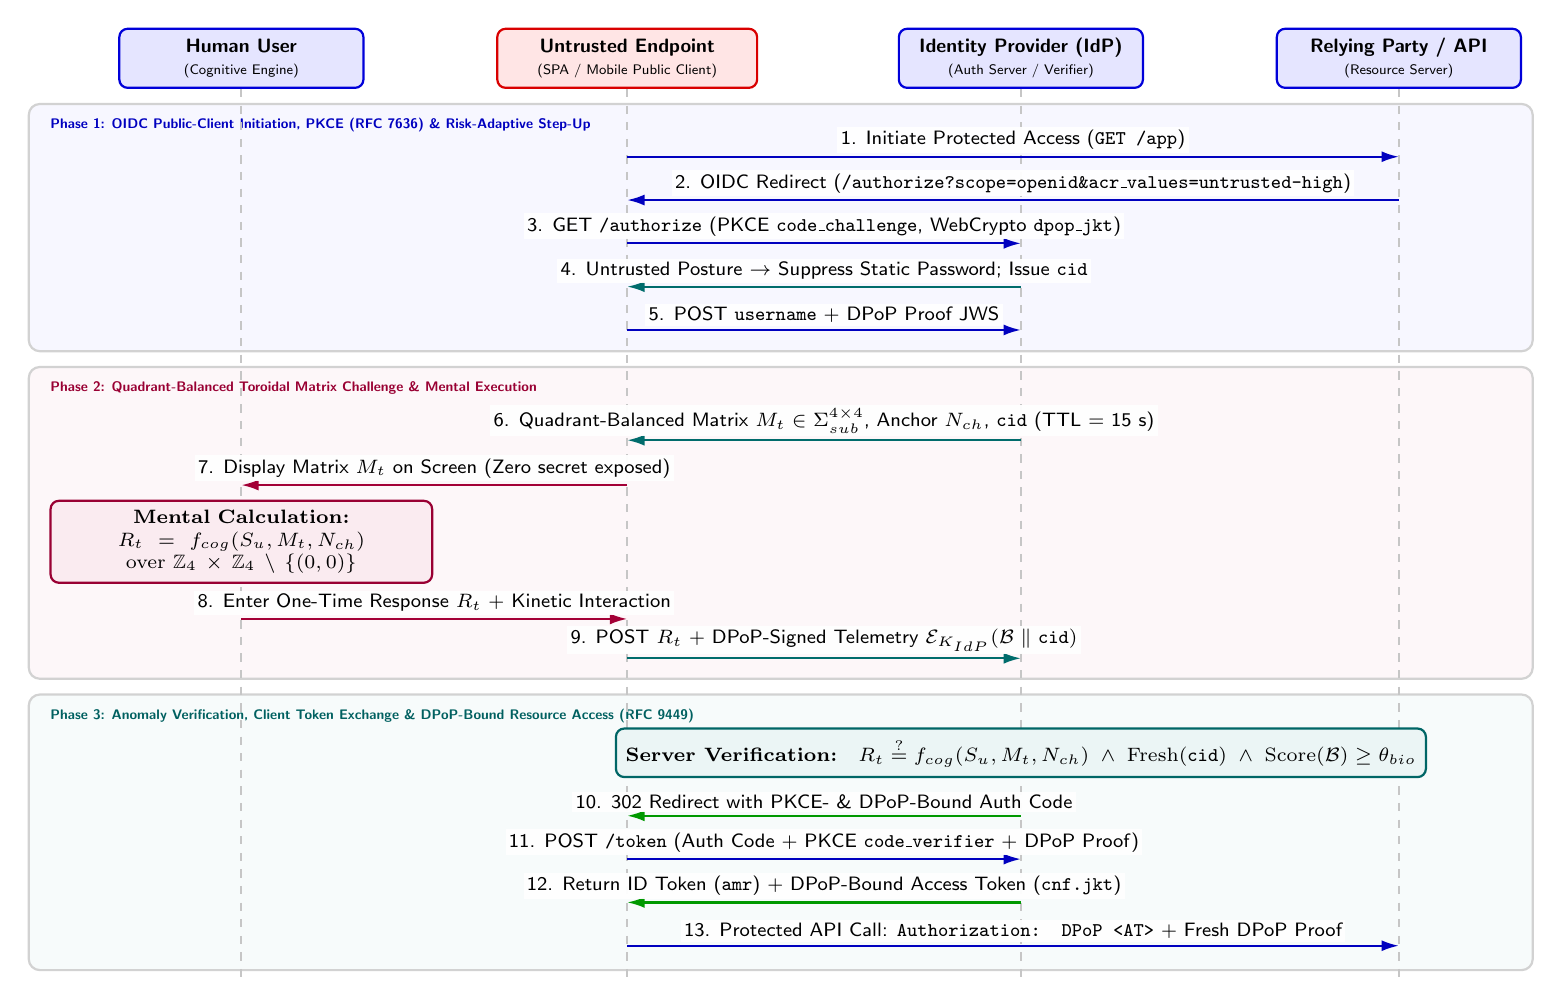
\begin{tikzpicture}[
    font=\sffamily\scriptsize,
    lifeline/.style={thick, dashed, draw=gray!45},
    actor/.style={rectangle, draw=blue!85!black, fill=blue!10, thick, minimum width=3.1cm, minimum height=0.75cm, align=center, rounded corners=3pt},
    untrusted/.style={rectangle, draw=red!85!black, fill=red!10, thick, minimum width=3.3cm, minimum height=0.75cm, align=center, rounded corners=3pt},
    phasebox/.style={rectangle, rounded corners=4pt, draw=gray!35, line width=0.8pt},
    lbl/.style={fill=white, fill opacity=0.95, text opacity=1, inner sep=1.2pt, font=\sffamily\scriptsize},
    msg/.style={-{Latex[length=2.2mm,width=1.4mm]}, thick, draw=blue!75!black},
    cogmsg/.style={-{Latex[length=2.2mm,width=1.4mm]}, thick, draw=purple!85!black},
    secmsg/.style={-{Latex[length=2.2mm,width=1.4mm]}, thick, draw=teal!85!black},
    retmsg/.style={-{Latex[length=2.2mm,width=1.4mm]}, thick, draw=green!60!black},
    cogbox/.style={rectangle, draw=purple!80!black, fill=purple!8, thick, font=\scriptsize, align=center, rounded corners=3pt, inner sep=3.5pt},
    idpbox/.style={rectangle, draw=teal!80!black, fill=teal!8, thick, font=\scriptsize, align=center, rounded corners=3pt, inner sep=3.5pt}
]
    % Phase background boxes with generous top header strips and left/right margins
    \draw[phasebox, fill=blue!3] (-2.7, -0.58) rectangle (16.4, -3.72);
    \node[anchor=north west, font=\sffamily\bfseries\tiny, color=blue!75!black] at (-2.55, -0.64) {\textsc{Phase 1: OIDC Public-Client Initiation, PKCE (RFC 7636) \& Risk-Adaptive Step-Up}};

    \draw[phasebox, fill=purple!3] (-2.7, -3.92) rectangle (16.4, -7.88);
    \node[anchor=north west, font=\sffamily\bfseries\tiny, color=purple!80!black] at (-2.55, -3.98) {\textsc{Phase 2: Quadrant-Balanced Toroidal Matrix Challenge \& Mental Execution}};

    \draw[phasebox, fill=teal!3] (-2.7, -8.08) rectangle (16.4, -11.58);
    \node[anchor=north west, font=\sffamily\bfseries\tiny, color=teal!75!black] at (-2.55, -8.14) {\textsc{Phase 3: Anomaly Verification, Client Token Exchange \& DPoP-Bound Resource Access (RFC 9449)}};

    % Lifeline headers
    \node[actor] (user) at (0, 0) {\textbf{Human User}\\\tiny(Cognitive Engine)};
    \node[untrusted] (client) at (4.9, 0) {\textbf{Untrusted Endpoint}\\\tiny(SPA / Mobile Public Client)};
    \node[actor] (idp) at (9.9, 0) {\textbf{Identity Provider (IdP)}\\\tiny(Auth Server / Verifier)};
    \node[actor] (rp) at (14.7, 0) {\textbf{Relying Party / API}\\\tiny(Resource Server)};

    % Lifeline paths
    \draw[lifeline] (user.south) -- ++(0, -11.30);
    \draw[lifeline] (client.south) -- ++(0, -11.30);
    \draw[lifeline] (idp.south) -- ++(0, -11.30);
    \draw[lifeline] (rp.south) -- ++(0, -11.30);

    % Phase 1: Steps 1 to 5
    \draw[msg] (4.9, -1.25) -- (14.7, -1.25) node[lbl, midway, above=1pt] {1. Initiate Protected Access (\texttt{GET /app})};
    \draw[msg] (14.7, -1.80) -- (4.9, -1.80) node[lbl, midway, above=1pt] {2. OIDC Redirect (\texttt{/authorize?scope=openid\&acr\_values=untrusted-high})};
    \draw[msg] (4.9, -2.35) -- (9.9, -2.35) node[lbl, midway, above=1pt] {3. GET \texttt{/authorize} (PKCE \texttt{code\_challenge}, WebCrypto \texttt{dpop\_jkt})};
    \draw[secmsg] (9.9, -2.90) -- (4.9, -2.90) node[lbl, midway, above=1pt] {4. Untrusted Posture $\rightarrow$ Suppress Static Password; Issue \texttt{cid}};
    \draw[msg] (4.9, -3.45) -- (9.9, -3.45) node[lbl, midway, above=1pt] {5. POST \texttt{username} + DPoP Proof JWS};

    % Phase 2: Steps 6 to 9
    \draw[secmsg] (9.9, -4.85) -- (4.9, -4.85) node[lbl, midway, above=1pt] {6. Quadrant-Balanced Matrix $M_t \in \Sigma_{sub}^{4\times 4}$, Anchor $N_{ch}$, \texttt{cid} (TTL = 15 s)};
    \draw[cogmsg] (4.9, -5.42) -- (0, -5.42) node[lbl, midway, above=1pt] {7. Display Matrix $M_t$ on Screen (Zero secret exposed)};
    \node[cogbox, text width=4.6cm] at (0, -6.14) {\textbf{Mental Calculation:}\\$R_t = f_{cog}(S_u, M_t, N_{ch})$ over $\mathbb{Z}_4 \times \mathbb{Z}_4 \setminus \{(0,0)\}$};
    \draw[cogmsg] (0, -7.12) -- (4.9, -7.12) node[lbl, midway, above=1pt] {8. Enter One-Time Response $R_t$ + Kinetic Interaction};
    \draw[secmsg] (4.9, -7.62) -- (9.9, -7.62) node[lbl, midway, above=1pt] {9. POST $R_t$ + DPoP-Signed Telemetry $\mathcal{E}_{K_{IdP}}(\mathcal{B} \parallel \texttt{cid})$};

    % Phase 3: Steps 10 to 13
    \node[idpbox] at (9.9, -8.82) {\textbf{Server Verification: } $R_t \stackrel{?}{=} f_{cog}(S_u, M_t, N_{ch}) \;\land\; \text{Fresh}(\texttt{cid}) \;\land\; \text{Score}(\mathcal{B}) \ge \theta_{bio}$};
    \draw[retmsg] (9.9, -9.62) -- (4.9, -9.62) node[lbl, midway, above=1pt] {10. 302 Redirect with PKCE- \& DPoP-Bound Auth Code};
    \draw[msg] (4.9, -10.17) -- (9.9, -10.17) node[lbl, midway, above=1pt] {11. POST \texttt{/token} (Auth Code + PKCE \texttt{code\_verifier} + DPoP Proof)};
    \draw[retmsg] (9.9, -10.72) -- (4.9, -10.72) node[lbl, midway, above=1pt] {12. Return ID Token (\texttt{amr}) + DPoP-Bound Access Token (\texttt{cnf.jkt})};
    \draw[msg] (4.9, -11.27) -- (14.7, -11.27) node[lbl, midway, above=1pt] {13. Protected API Call: \texttt{Authorization: DPoP <AT>} + Fresh DPoP Proof};
\end{tikzpicture}%
}
\caption{Standards-compliant OIDC Core 1.0, RFC 7636 PKCE, and RFC 9449 DPoP protocol exchange for BC-MFA public clients.}
\label{fig:bcmfa_flow}
\end{figure*}

\subsection{Cognitive Challenge and Toroidal Transformation Mechanics}
The core visual defense of BC-MFA relies on quadrant-balanced permutation matrices with controlled symbol multiplicity, ensuring that display scrapers extract minimal usable intelligence regarding the user's secret $S_u$. Upon step-up initiation, the IdP synthesizes an ephemeral challenge matrix $M_t$ of dimensions $4 \times 4$ ($N = 16$ cells) from an alphanumeric alphabet $\Sigma$ ($|\Sigma| = 36$), partitioned into $L = 4$ disjoint $2 \times 2$ quadrants ($Q_1$--$Q_4$). To balance instantaneous display entropy against multi-session intersection ambiguity, the server samples an active symbol subset $\Sigma_{sub} \subset \Sigma$ of cardinality $|\Sigma_{sub}| = N / d$ and assigns each symbol exact multiplicity $d = L = 4$ under \textit{quadrant-balanced placement}: every symbol in $\Sigma_{sub}$ appears exactly once inside each of the $L$ quadrants. The exact Shannon entropy of a balanced $L$-block challenge matrix $M_t$ (with $d = L$) is:
\begin{equation}
H_{\text{bal}}(M_t) = \log_2 \binom{|\Sigma|}{N/d} + d \cdot \log_2 \!\left( \left(\frac{N}{d}\right)! \right)
\label{eq:entropy}
\end{equation}
In the BC-MFA quadrant-balanced regime ($|\Sigma| = 36, N = 16, d = L = 4$), Eq.~(\ref{eq:entropy}) yields $H_{\text{bal}}(M_t) = \log_2 \binom{36}{4} + 4 \cdot \log_2(4!) \approx 15.85 + 18.34 = 34.19\text{ bits}$ of per-session challenge entropy (compared to $55.45\text{ bits}$ for half-balanced $d = L = 2$, $41.76\text{ bits}$ for unconstrained multiset placement $\log_2\binom{36}{4} + \log_2(16!/(4!)^4)$ with $d = 4$, and $82.72\text{ bits}$ for unconstrained full-alphabet i.i.d. placement $16 \log_2 36$). The server pairs $M_t$ with a public anchor character $N_{ch} \in \Sigma_{sub}$, a unique challenge identifier \texttt{cid}, and a strict expiration window ($\text{TTL} = 15\text{ s}$).

During trusted-device enrollment, the server assists the user in sampling a uniform random secret $S_u = \big(q_u, \langle (\Delta r_1, \Delta c_1), \dots, (\Delta r_{|R|}, \Delta c_{|R|}) \rangle\big)$ to eliminate human spatial selection bias. Secret $S_u$ comprises a private anchor quadrant $q_u \in \{Q_1, Q_2, Q_3, Q_4\}$ and an ordered sequence of $|R| = 4$ distinct \emph{non-zero} toroidal offset vectors in $\mathbb{Z}_4 \times \mathbb{Z}_4 \setminus \{(0,0)\}$. Explicitly excluding the identity offset $(0,0)$ is cryptographically necessary: otherwise $M_t[r_0, c_0] = N_{ch}$ would deterministically echo the public anchor character in every session, leaking that offset index immediately. Because $N_{ch}$ appears once in every quadrant, the user locates $N_{ch}$ within private quadrant $q_u$ to establish the session origin $(r_0, c_0) \in \mathbb{Z}_4 \times \mathbb{Z}_4$ without touching or hovering over it, then derives response $R_t = (s_1, \dots, s_{|R|})$:
\begin{equation}
s_i = M_t\big[(r_0 + \Delta r_i) \bmod 4,\; (c_0 + \Delta c_i) \bmod 4\big]
\label{eq:toroidal}
\end{equation}
for $i \in \{1, \dots, |R|\}$. Because modular addition in $\mathbb{Z}_4 \times \mathbb{Z}_4$ forms a bijection, distinct non-zero offsets map deterministically to distinct grid cells without boundary overflow. Figure~\ref{fig:worked_example} illustrates a complete step-by-step evaluation.

\begin{figure}[!t]
\centering
\resizebox{\columnwidth}{!}{%
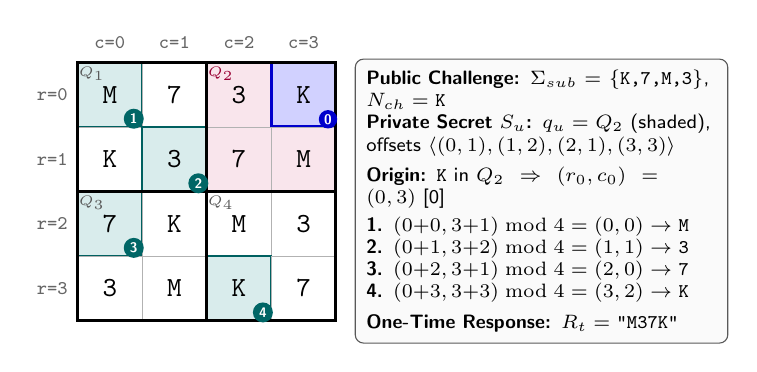
\begin{tikzpicture}[
    font=\sffamily\scriptsize,
    cell/.style={rectangle, draw=gray!60, minimum size=0.82cm, align=center, font=\ttfamily\bfseries\normalsize},
    qfill/.style={fill=purple!10},
    anc/.style={fill=blue!18, draw=blue!80!black, very thick},
    hit/.style={fill=teal!15, draw=teal!75!black, thick},
    badge/.style={circle, fill=teal!80!black, text=white, font=\sffamily\bfseries\tiny, inner sep=1pt}
]
    % Column indices
    \foreach \c in {0,1,2,3} {
        \node[font=\ttfamily\scriptsize, color=gray!80!black] at (\c*0.82 + 0.41, 0.25) {c=\c};
    }
    % Row indices
    \foreach \r in {0,1,2,3} {
        \node[font=\ttfamily\scriptsize, color=gray!80!black] at (-0.32, -\r*0.82 - 0.41) {r=\r};
    }

    % Grid cells: M = [['M','7','3','K'], ['K','3','7','M'], ['7','K','M','3'], ['3','M','K','7']]
    % Row 0
    \node[cell, hit] (c00) at (0*0.82+0.41, -0*0.82-0.41) {M};
    \node[cell]      (c01) at (1*0.82+0.41, -0*0.82-0.41) {7};
    \node[cell, qfill] (c02) at (2*0.82+0.41, -0*0.82-0.41) {3};
    \node[cell, anc]   (c03) at (3*0.82+0.41, -0*0.82-0.41) {K};
    % Row 1
    \node[cell]      (c10) at (0*0.82+0.41, -1*0.82-0.41) {K};
    \node[cell, hit] (c11) at (1*0.82+0.41, -1*0.82-0.41) {3};
    \node[cell, qfill] (c12) at (2*0.82+0.41, -1*0.82-0.41) {7};
    \node[cell, qfill] (c13) at (3*0.82+0.41, -1*0.82-0.41) {M};
    % Row 2
    \node[cell, hit] (c20) at (0*0.82+0.41, -2*0.82-0.41) {7};
    \node[cell]      (c21) at (1*0.82+0.41, -2*0.82-0.41) {K};
    \node[cell]      (c22) at (2*0.82+0.41, -2*0.82-0.41) {M};
    \node[cell]      (c23) at (3*0.82+0.41, -2*0.82-0.41) {3};
    % Row 3
    \node[cell]      (c30) at (0*0.82+0.41, -3*0.82-0.41) {3};
    \node[cell]      (c31) at (1*0.82+0.41, -3*0.82-0.41) {M};
    \node[cell, hit] (c32) at (2*0.82+0.41, -3*0.82-0.41) {K};
    \node[cell]      (c33) at (3*0.82+0.41, -3*0.82-0.41) {7};

    % Bold quadrant dividers
    \draw[very thick, black] (0, 0) rectangle (3.28, -3.28);
    \draw[very thick, black] (1.64, 0) -- (1.64, -3.28);
    \draw[very thick, black] (0, -1.64) -- (3.28, -1.64);

    % Quadrant labels
    \node[font=\sffamily\tiny\bfseries, color=gray!70!black] at (0.18, -0.14) {$Q_1$};
    \node[font=\sffamily\tiny\bfseries, color=purple!80!black] at (1.82, -0.14) {$Q_2$};
    \node[font=\sffamily\tiny\bfseries, color=gray!70!black] at (0.18, -1.78) {$Q_3$};
    \node[font=\sffamily\tiny\bfseries, color=gray!70!black] at (1.82, -1.78) {$Q_4$};

    % Step badges
    \node[badge] at ($(c00.south east)+(-0.12,0.12)$) {1};
    \node[badge] at ($(c11.south east)+(-0.12,0.12)$) {2};
    \node[badge] at ($(c20.south east)+(-0.12,0.12)$) {3};
    \node[badge] at ($(c32.south east)+(-0.12,0.12)$) {4};
    \node[circle, fill=blue!80!black, text=white, font=\sffamily\bfseries\tiny, inner sep=0.8pt] at ($(c03.south east)+(-0.12,0.12)$) {0};

    % Right-hand explanation box
    \node[rectangle, draw=black!65, fill=gray!4, rounded corners=3pt, align=left, font=\sffamily\scriptsize\raggedright, anchor=north west, inner sep=4pt, text width=4.45cm] at (3.52, 0.05) {
        \textbf{Public Challenge:} $\Sigma_{sub}=\{\texttt{K,7,M,3}\}$, $N_{ch}=\texttt{K}$\\
        \textbf{Private Secret $S_u$:} $q_u = Q_2$ (shaded),\\
        offsets $\langle (0,1),(1,2),(2,1),(3,3)\rangle$\\[3pt]
        \textbf{Origin:} \texttt{K} in $Q_2 \Rightarrow (r_0,c_0)=(0,3)$~\textsf{[0]}\\[2pt]
        \textbf{1.} $(0{+}0,3{+}1)\bmod 4=(0,0)\rightarrow \texttt{M}$\\
        \textbf{2.} $(0{+}1,3{+}2)\bmod 4=(1,1)\rightarrow \texttt{3}$\\
        \textbf{3.} $(0{+}2,3{+}1)\bmod 4=(2,0)\rightarrow \texttt{7}$\\
        \textbf{4.} $(0{+}3,3{+}3)\bmod 4=(3,2)\rightarrow \texttt{K}$\\[3pt]
        \textbf{One-Time Response:} $R_t = \texttt{"M37K"}$
    };
\end{tikzpicture}%
}
\caption{Worked example of a $4 \times 4$ quadrant-balanced toroidal challenge ($d=L=4$) illustrating private origin anchoring and modular wrap-around.}
\label{fig:worked_example}
\end{figure}

Because $M_t$ refreshes independently on every attempt with a newly sampled subset $\Sigma_{sub} \subset \Sigma$, consecutive responses for a fixed secret $S_u$ almost never repeat. Even under a worst-case analytical lower bound where $\Sigma_{sub}$ were held fixed across sessions (i.i.d. symbol approximation), divergence satisfies:
\begin{equation}
\Pr\big(R_{t_1} \ne R_{t_2} \;\big|\; S_u, \Sigma_{sub}\text{ fixed}\big) \approx 1 - \left(\frac{d}{N}\right)^{|R|} = \frac{255}{256}
\label{eq:divergence}
\end{equation}
($99.61\%$ analytical; $99.46\%$ empirically under exact finite-grid quadrant-balanced sampling without replacement). When $\Sigma_{sub}$ is resampled uniformly from $|\Sigma|=36$ each session, consecutive responses diverge with empirical probability $99.999\%$ (measured across $2 \times 10^5$ independent pairs), since matching requires the new 4-symbol subset to contain every distinct character in $R_{t_1}$.

\subsection{Passive Behavioral Anomaly Telemetry}
To deter automated replay bots and off-device human solver relays, the client runs a passive event observer during the challenge ceremony. On desktop browsers, the observer samples pre-entry cognitive hesitation latency ($\tau_{cog}$), pointer trajectory curvature ($\kappa_{path}$), velocity inflections ($\vec{v}_p$), keystroke hold times ($HT_i = t_{up,i} - t_{down,i}$), and inter-key flight times ($FT_i = t_{down,i+1} - t_{up,i}$), yielding $\mathcal{B}_{desktop} = \{\tau_{cog}, \vec{v}_p, \kappa_{path}, HT, FT\}$~\cite{khan2024mouse}. On mobile touchscreens where continuous cursor paths are absent, it records $\mathcal{B}_{mobile} = \{\tau_{cog}, A_{touch}, P_{touch}, HT, FT\}$ capturing contact area and normalized capacitive pressure~\cite{incel2021dakota}.

Crucially, we recognize a fundamental statistical boundary: a 4-character response yields only 4 hold times and 3 flight times, and untrusted kiosks exhibit heterogeneous keyboards, pointer DPIs, and browser event throttling. Consequently, BC-MFA does \emph{not} rely on 4-keystroke cadence for standalone cross-device biometric user identification. Instead, $\text{Score}(\mathcal{B})$ operates primarily as a \emph{human-vs-automation and relay anomaly detector} (flagging zero-hesitation scripted injections, uniform synthetic timing, or out-of-band relay delays), applying user-specific baseline scoring strictly as a secondary risk signal on previously enrolled devices.

To prevent cross-session telemetry replay and passive network inspection, the client binds the active challenge identifier \texttt{cid} inside the payload, signs the hash with its ephemeral WebCrypto DPoP private key, and encrypts $\mathcal{E}_{K_{IdP}}(\mathcal{B} \parallel \texttt{cid})$ under the IdP's public key. Note that payload encryption protects confidentiality on the wire rather than against local client tampering; integrity against scripted spoofing rests on server-side challenge timing bounds and Isolation Forest / Random Forest anomaly scoring ($\text{Score}(\mathcal{B}) \ge \theta_{bio}$).

\subsection{OpenID Connect Profile, RFC 8176 Claims, and RFC 9449 DPoP}
When both $R_t$ and $\text{Score}(\mathcal{B})$ pass verification within the 15-second TTL, the IdP issues a PKCE- and DPoP-bound authorization code. Following RFC 9700 for public SPA/mobile clients~\cite{rfc9700bcp}, the \emph{client} exchanges the authorization code directly at the IdP \texttt{/token} endpoint presenting both PKCE \texttt{code\_verifier} and a fresh DPoP Proof JWS signed by its non-exportable WebCrypto private key (\texttt{extractable: false}, stored in \texttt{IndexedDB}). The IdP returns: (1) an OpenID Connect Core 1.0 ID Token~\cite{oidc_core1} populated with \emph{standard registered} RFC 8176 \texttt{amr} values~\cite{rfc8176amr}—\texttt{"mfa"} (multi-factor), \texttt{"kba"} (cognitive knowledge-based challenge), \texttt{"rba"} (risk-based behavioral anomaly verification), and \texttt{"swk"} (software-secured proof-of-possession key)—ensuring zero mandatory code changes for standard Relying Parties, plus an optional namespaced extension claim for BC-MFA-aware RPs; and (2) an RFC 9449 DPoP-bound Access Token carrying the \texttt{cnf.jkt} JWK SHA-256 thumbprint~\cite{rfc9449dpop} validated by the Resource Server on every API request. Listing~\ref{lst:oidc_token} presents both decoded synthetic JWT payloads.

\noindent\begin{minipage}{\columnwidth}
\begin{lstlisting}[caption={Decoded OIDC ID Token (Registered RFC 8176 AMR) and RFC 9449 DPoP-Bound Access Token Confirmation Claims}, label={lst:oidc_token}, basicstyle=\ttfamily\scriptsize, numbers=none]
// 1. OIDC ID Token Payload (RFC 8176 Standard AMR)
{
  "iss": "https://identity.ispgaya.pt/auth",
  "sub": "usr-2022105675-casousa",
  "aud": "sistemas-web-mobile-app",
  "exp": 1794502800, "iat": 1794499200,
  "auth_time": 1794499195,
  "nonce": "n-0S6_WzA2MjY",
  "acr": "urn:ispgaya:oidc:acr:untrusted-high",
  "amr": ["mfa", "kba", "rba", "swk"],
  "https://identity.ispgaya.pt/bc_mfa": {
    "posture": "untrusted", "cognitive_ms": 3820,
    "anomaly_score": 0.94
  }
}
// 2. DPoP-Bound Access Token Claims (RFC 9449)
{
  "iss": "https://identity.ispgaya.pt/auth",
  "sub": "usr-2022105675-casousa",
  "scope": "openid api.read",
  "cnf": {
    "jkt": "0ZcOCORZNYy-DWpqq30jZyJGHTN0d2HglBV3uiguA4I"
  }
}
\end{lstlisting}
\end{minipage}

\section{Security and Threat Analysis}
\label{sec:security_analysis}

\subsection{Threat Model and Adversary Capabilities}
We evaluate the security boundaries of BC-MFA under a host-compromise threat model mapped to the MITRE ATT\&CK taxonomy as formalized in recent phishing and credential-theft studies~\cite{lain2022phishing, lee2024beneath, lim2025phishers}. The adversary is assumed to hold unprivileged, user-space code execution on the client endpoint via drive-by downloads or spear-phishing payloads~\cite{lain2022phishing}, commanding five exploitation vectors: input logging (T1056.001) capturing keyboard/touch events; screen capture (T1113) recording desktop frames; carrier-level SIM swapping targeting telephonic factors~\cite{nahapetyan2024sms}; network-level AitM reverse proxying (T1557) mediating TLS traffic~\cite{kondracki2021catching}; and automated bot replay or bearer session-token theft (T1059, T1539)~\cite{hilbig2023protect}.

We demarcate explicit epistemic limits. BC-MFA defends against commodity user-space infostealers that log keystrokes, scrape screens, and exfiltrate cached files or bearer cookies. We do \emph{not} claim defense against adversaries holding administrative kernel privileges (ring 0) or actively attaching same-privilege browser-debugging sessions (e.g., Chrome DevTools Protocol or malicious browser extensions) capable of invoking live WebCrypto handles as signing oracles, because full runtime control over the browser process undermines all purely software-based client isolation. Table~\ref{tab:security_comparison} summarizes the comparative security posture across paradigms.

\begin{table*}[!t]
\caption{Comparative Resilience of Authentication Paradigms on Untrusted Endpoints}
\label{tab:security_comparison}
\centering
\resizebox{\textwidth}{!}{%
\begin{tabular}{@{}lcccccc@{}}
\toprule
\textbf{Authentication Paradigm} & \textbf{Keylogger (T1056)} & \textbf{Screen Capture (T1113)} & \textbf{SIM Swapping} & \textbf{AitM Proxy (T1557)} & \textbf{Session Theft (T1539)} & \textbf{Zero Hardware} \\
\midrule
Static Password & No & No & Immune & No (Relayed) & No (Bearer) & Yes \\
SMS / TOTP (RFC 6238)~\cite{rfc6238totp} & Partial (TTL) & No (Direct view) & Vulnerable (SMS) & No (Relayed) & No (Bearer) & Yes \\
Mobile Push / Number Match~\cite{jubur2025usability} & Yes (OOB) & No (DOM prompt) & Immune & No (Relayed) & No (Bearer) & Partial (Phone) \\
FIDO2 / WebAuthn~\cite{angelogianni2024how, w3cwebauthn3} & Yes (PubKey) & Yes (No secret) & Immune & Yes (Origin bound) & Needs DPoP/DBSC & No (Token) \\
\textbf{BC-MFA (Proposed)} & \textbf{Yes (One-time $R_t$)} & \textbf{Yes (Blind $M_t{+}q_u$)} & \textbf{Immune (No SMS)} & \textbf{High* (Pinning+TTL)} & \textbf{High (RFC 9449)} & \textbf{Yes} \\
\bottomrule
\multicolumn{7}{@{}l}{\footnotesize *Mitigates automated relay/solver farms and enrolled-browser proxies via DPoP key pinning; first-contact active reverse proxies remain outside software-only scope (Section~\ref{sec:security_analysis}-D).}
\end{tabular}%
}
\end{table*}

\subsection{Resistance Against Input Logging, Screen Scraping, and SIM Swapping}
BC-MFA eliminates telephonic carriers entirely, providing structural immunity to SIM swapping and SS7 interception campaigns~\cite{nahapetyan2024sms}. On compromised hosts, static passwords are suppressed and keyloggers capture only the ephemeral one-time response $R_t$, which holds zero replay utility once the 15-second challenge expires:
\begin{equation}
\Pr\big(R_t \text{ is valid at } t + \Delta t \;\big|\; \Delta t > \text{TTL}\big) = 0
\label{eq:ttl}
\end{equation}
If the adversary captures the screen (T1113), the frame exposes only matrix $M_t$ and public anchor character $N_{ch}$. Because the identity offset $(0,0)$ is excluded from $\mathbb{Z}_4 \times \mathbb{Z}_4$, reconstructing the ordered 4-offset path requires searching the combinatorial space of distinct non-zero $|R|$-permutations over $N - 1 = 15$ valid offsets:
\begin{equation}
\Omega = \frac{(N - 1)!}{(N - 1 - |R|)!} = \frac{15!}{11!} = 32{,}760
\label{eq:omega}
\end{equation}
Combined with the private anchor quadrant $q_u \in \{1, \dots, L\}$ ($L = 4$), the adversary's full initial hypothesis space is $|\mathcal{C}_0| = L \cdot \Omega = 4 \times 32{,}760 = 131{,}040$ candidate secrets $(q_u, \text{path})$.

\subsection{Multi-Session Intersection Analysis and Monte Carlo Validation}
A persistent host-level infostealer observing $k$ consecutive logins records pairs $\{(M_1, R_1), \dots, (M_k, R_k)\}$ to intersect consistent secrets~\cite{binbeshr2025challenge}. Crucially, we model a \emph{rational consistent adversary} who exploits the fact that the user's quadrant $q_u$ remains fixed across sessions: the attacker filters the full hypothesis space $|\mathcal{C}_0| = L \cdot \Omega = 131{,}040$ by testing each pair $(q, \text{path})$ against all $k$ sessions simultaneously. Under an i.i.d. symbol approximation where each wrong hypothesis survives an independent session with probability $(d/N)^{|R|} = (4/16)^4 = 1/256$, the expected surviving candidate set after $k$ compromised sessions is approximated by:
\begin{equation}
\mathbb{E}\big[|\mathcal{C}_k|\big] \approx 1 + \big(L \cdot \Omega - 1\big) \cdot \left(\frac{d}{N}\right)^{k|R|}
\label{eq:intersection}
\end{equation}
For $N = 16, d = L = 4, |R| = 4$, Eq.~(\ref{eq:intersection}) predicts an i.i.d. baseline of $512.9$ candidates at $k = 1$, $3.00$ at $k = 2$, and collapse toward $1.01$ at $k = 3$.

To capture exact finite-grid dependencies under balanced placement without replacement, we executed a reproducible 500-trial Monte Carlo simulation in Python (fixed PRNG \texttt{seed = 2026}, rational consistent adversary tracking $(q, \text{path})$ over $L \cdot \Omega$, publicly available at \url{https://github.com/casousavng/bc-mfa-oidc}) across $k \in \{1, 2, 3, 4\}$ sessions for three regimes: naive $(d=1, L=1)$, half-balanced $(d=2, L=2)$, and quadrant-balanced BC-MFA $(d=4, L=4)$. Because surviving candidate distributions are strongly right-skewed, Table~\ref{tab:mc_results} reports mean $\pm$ SD alongside the median, 5th percentile ($\text{P}_5$, representing worst-case attacker luck), and exact secret recovery rate $\Pr(|\mathcal{C}_k| = 1)$.

\begin{table}[!t]
\caption{500-Trial Rational-Adversary Monte Carlo Intersection Results (\texttt{seed=2026}, $(0,0)$ Excluded)}
\label{tab:mc_results}
\centering
\scriptsize
\setlength{\tabcolsep}{3.5pt}
\begin{tabular}{@{}lcccc@{}}
\toprule
\textbf{Regime ($d, L$)} & \textbf{$k$} & \textbf{Mean $\pm$ SD} & \textbf{Med. / $\text{P}_5$} & \textbf{$\Pr(|\mathcal{C}_k|{=}1)$} \\
\midrule
Naive ($1, 1$) & 1 & $1.00 \pm 0.00$ & 1.0 / 1 & 100.0\% \\
\midrule
Half-Bal. ($2, 2$) & 1 & $22.16 \pm 8.61$ & 16.0 / 8 & 0.0\% \\
Half-Bal. ($2, 2$) & 2 & $1.51 \pm 0.98$ & 1.0 / 1 & 66.6\% \\
Half-Bal. ($2, 2$) & 3 & $1.05 \pm 0.25$ & 1.0 / 1 & 95.2\% \\
\midrule
\textbf{BC-MFA ($4, 4$)} & \textbf{1} & \textbf{$579.26 \pm 161.97$} & \textbf{576.0 / 288} & \textbf{0.0\%} \\
\textbf{BC-MFA ($4, 4$)} & \textbf{2} & \textbf{$10.44 \pm 16.31$} & \textbf{6.0 / 2} & \textbf{1.6\%} \\
BC-MFA ($4, 4$) & 3 & $1.75 \pm 1.49$ & 1.0 / 1 & 56.6\% \\
BC-MFA ($4, 4$) & 4 & $1.15 \pm 0.38$ & 1.0 / 1 & 86.2\% \\
\bottomrule
\end{tabular}
\end{table}

Table~\ref{tab:mc_results} exposes a decisive operational threshold. In the naive baseline, a single capture compromises the secret deterministically ($100\%$). In the intermediate $(2, 2)$ regime, two sessions yield $66.6\%$ exact recovery. In BC-MFA $(4, 4)$, finite-grid quadrant balance sustains higher ambiguity than the i.i.d. approximation ($576$ median and $288$ $\text{P}_5$ at $k = 1$; $6.0$ median and $2$ $\text{P}_5$ at $k = 2$, with only $1.6\%$ exact recovery), but session $k = 3$ causes recovery to jump sharply to $56.6\%$. Therefore, the IdP enforces a strict policy ceiling of $k_{\max} = 2$ untrusted step-up logins (or $k_{\max} = 1$ with $0.0\%$ recovery for maximum-assurance profiles), requiring a trusted-device secret re-enrollment before permitting further untrusted sessions—avoiding fragile mental offset shifts over untrusted channels.

\subsection{Mitigation and Boundaries Against AitM Reverse Proxies}
We analyze three distinct AitM reverse-proxy scenarios (e.g., Evilginx~\cite{kondracki2021catching, lim2025phishers}):
\begin{enumerate}
    \item \textit{Automated Relay or Remote Solver Farm:} Intercepting $M_t$ and forwarding it to an automated optical bot or remote human solver induces sharp timing and kinematic anomalies—either near-zero hesitation ($\tau_{cog} \approx 0$) with uniform synthetic cadence or network-plus-comprehension latency exceeding the 15-second TTL—triggering rejection ($\text{Score}(\mathcal{B}) < \theta_{bio}$)~\cite{khan2024mouse}.
    \item \textit{Active Proxy on a Previously Enrolled Browser:} When the browser already holds a non-exportable WebCrypto DPoP keypair (\texttt{extractable: false}) stored in \texttt{IndexedDB} under the legitimate IdP origin, Same-Origin Policy prevents a spoofed domain (\texttt{login.evil-proxy.example}) from accessing the pinned key, causing the IdP to reject the mismatched \texttt{dpop\_jkt} and \texttt{htu} (HTTP URI) signature~\cite{rfc9449dpop}.
    \item \textit{Active Proxy on a First-Contact Public Kiosk (Explicit Boundary):} When a user visits a spoofed phishing domain from an unpinned kiosk with no prior DPoP key, an active reverse proxy capable of rewriting client-side JavaScript in transit can generate its own server-side DPoP keypair toward the IdP, terminating sender constraint on the proxy. We state this limitation candidly: deterministic first-contact phishing resistance without prior origin pinning requires browser-enforced, hardware-backed origin binding (WebAuthn). Even on unpinned kiosks, however, once the user connects to the authentic IdP origin, RFC 9449 DPoP binding and RFC 7636 PKCE block passive infostealers from replaying exfiltrated authorization codes or access tokens from external attacker hosts~\cite{rfc7636pkce, rfc9449dpop, rfc9700bcp}.
\end{enumerate}

\section{Usability, Fault Tolerance, and Operational Scope}
\label{sec:usability_and_overhead}

\subsection{Analytical Cognitive Latency Envelope}
Cognitive authentication architectures must remain within acceptable human completion bounds while preserving narrow cryptographic expiration windows~\cite{kepkowski2023challenges, binbeshr2025challenge}. Prior to human-subject testing, we establish a literature-derived additive latency envelope adapted from grid-based challenge-response studies~\cite{binbeshr2025challenge, duzgun2022shoulder}:
\begin{equation}
T_{total} = T_{perceptual} + T_{cognitive} + T_{motor}
\label{eq:latency}
\end{equation}
Perceptual search $T_{perceptual}$ spans $0.35\text{ s}$ to $0.60\text{ s}$ to locate $N_{ch}$ inside the 4-cell quadrant $q_u$. Cognitive traversal $T_{cognitive}$ estimates mental execution across four toroidal offsets at $450\text{ ms}$ to $725\text{ ms}$ per step ($1.80\text{ s}$ to $2.90\text{ s}$)~\cite{binbeshr2025challenge}. Physical input $T_{motor}$ for a 4-character string averages $1.10\text{ s}$ to $1.50\text{ s}$~\cite{incel2021dakota, khan2024mouse}. Aggregating these components yields an analytical mean target of $3.25\text{ s}$ to $5.00\text{ s}$, comfortably inside the 15-second TTL. Because toroidal wrap-around ($\bmod 4$) may impose higher mental load during initial onboarding than linear grid lookups, empirical validation across trained and novice cohorts is prioritized in Section~\ref{sec:experimental_design_and_thesis}.

\subsection{Error Rates, Retention, and Hardware-Free Recovery}
Empirical evaluations of shoulder-surfing-resistant challenge-response and graphical PIN schemes report initial human entry error rates between $4\%$ and $8\%$, alongside recall latency growth after multi-week inactivity~\cite{binbeshr2025challenge, duzgun2022shoulder}. To balance fault tolerance with intersection safety, BC-MFA enforces a layered verification policy. Upon a single algebraic mismatch ($R_t \ne R_{expected}$), the IdP issues one immediate retry on a fresh matrix $M_{t+1}$ without incrementing the untrusted intersection counter, provided behavioral telemetry confirms human liveness (failed submissions leak no valid $(M_t, R_t)$ pair to scrapers). If hesitation exceeds $\tau_{cog} > 6.0\text{ s}$, the UI can display a user-enrolled semantic mnemonic cue that aids path recall without revealing grid coordinates.

If response $R_t$ is valid but the behavioral score falls within a marginal uncertainty band ($\theta_{bio} - \epsilon \le \text{Score}(\mathcal{B}) < \theta_{bio}$), the IdP requests one confirmatory matrix rather than locking the session. After two consecutive cognitive failures, rather than falling back to vulnerable SMS OTP or mandating a corporate managed phone (which would contradict hardware independence and reopen recovery flaws documented by Amft et al.~\cite{amft2023weve}), the IdP enforces exponential cooldown throttling and routes account recovery to policy-selected strong channels: trusted-device re-authentication, pre-printed single-use cryptographic recovery codes, or electronic identity (eID) verification following Schwarz et al.~\cite{schwarz2022feido}.

\subsection{Enrollment Bias, Accessibility, and Application Scope}
Allowing users to choose their own offset paths induces predictable spatial patterns (e.g., linear horizontal sweeps) that shrink effective secret entropy well below $\Omega = 32{,}760$. BC-MFA therefore employs server-assisted uniform random secret generation paired with interactive visual mnemonic onboarding on a trusted device. Furthermore, because visual-spatial modular arithmetic under a 15-second window creates barriers for users with visual, motor, or cognitive disabilities, enterprise deployments must treat BC-MFA as an optional step-up authenticator paired with WCAG-compliant alternatives (such as hardware passkeys or audio-tactile schemes) rather than a universal mandatory replacement~\cite{mahfouz2025passkeys}. Its primary operational scope is targeted, hardware-free Step-Up defense on unmanaged BYOD endpoints, shared university or hospital terminals, and public kiosks where resident user-space infostealers threaten routine password or OTP entry.

\section{Experimental Design and Empirical Evaluation Plan}
\label{sec:experimental_design_and_thesis}

\subsection{Formal Research Hypotheses}
To validate the operational viability of BC-MFA within the author's Master's dissertation at ISPGAYA, we formulate three falsifiable hypotheses:
\begin{align}
H_1: &\quad \mu_{T_{total}} \le 5.0\text{ s},\;\; \sigma_{T} \le 1.25\text{ s} \label{eq:h1}\\
H_2: &\quad \text{SUS} \ge 75.0,\;\; \text{NASA-TLX}_{mental} \le 40.0 \label{eq:h2}\\
H_3: &\quad \text{FAR}_{bot/relay} \le 1.5\%,\;\; \text{FRR}_{human} \le 4.0\% \label{eq:h3}
\end{align}
Hypothesis $H_1$ posits that trained participants complete perceptual search, toroidal traversal, and 4-character input within five seconds on average. Hypothesis $H_2$ tests whether the ceremony achieves acceptable enterprise usability (SUS $\ge 75$) without excessive mental workload (NASA-TLX mental demand $\le 40$). Hypothesis $H_3$ evaluates whether the passive behavioral anomaly classifier separates legitimate human cognitive ceremonies from automated replay bots and off-device relay solvers across heterogeneous desktop and mobile endpoints within strict error tolerances.

\subsection{Testbed Implementation Architecture}
The experimental prototype comprises three modular tiers. The server tier implements a custom Authenticator SPI for Keycloak 24 handling HSM-backed secret storage, quadrant-balanced matrix synthesis, RFC 7636 PKCE validation, RFC 9449 DPoP verification, and OIDC token issuance with registered RFC 8176 \texttt{amr} claims. The client tier consists of a TypeScript SPA web agent and a React Native mobile application with non-blocking WebCrypto DPoP key management and passive interaction observers. The analytics tier runs a Scikit-Learn service executing Isolation Forest and Random Forest anomaly scoring over $\mathcal{B}$.

\subsection{Longitudinal Human Study, Ethics, and Statistical Design}
The empirical study will recruit $N = 64$ participants stratified equally across technical and non-technical backgrounds. An a priori statistical power analysis for repeated-measures ANOVA across four longitudinal timepoints (medium effect size $f = 0.25$, $\alpha = 0.05$, sphericity correction $\epsilon = 0.75$) confirms that $N = 64$ provides statistical power $1 - \beta > 0.90$ even after $15\%$ attrition. All procedures will obtain Institutional Ethics Board (IRB) approval prior to recruitment, enforcing informed consent and strict GDPR Art.~9 compliance (pseudonymized participant IDs, ephemeral kinetic feature retention, and explicit opt-out rights).

The protocol spans four milestones: trusted-device onboarding with interactive tutorial, immediate post-training verification, 7-day recall, and 30-day retention, employing a counterbalanced within-subjects baseline against TOTP (RFC 6238) and WebAuthn passkeys. Repeated-measures ANOVA with Greenhouse-Geisser sphericity corrections will quantify completion latency, cognitive error decay, and False Reject Rates across sessions.

\subsection{Adversarial Red-Team Emulation and Ablation}
Host-compromise survivability will be tested empirically against two controlled red-team harnesses. First, an Evilginx 3.x reverse proxy will execute automated relay, remote solver-farm, enrolled-browser pinning, and first-contact phishing scenarios to validate both timing/pinning mitigations and the documented first-contact boundary. Second, user-space infostealer harnesses modeling RedLine and Lumma will capture input and display buffers under two modes: (a) an \emph{ablation mode} with the $k_{\max} = 2$ policy ceiling intentionally disabled across 100 consecutive sessions to measure empirical rule-set shrinkage $|\mathcal{C}_k|$ against Table~\ref{tab:mc_results}, and (b) \emph{production enforcement mode} verifying deterministic blocking once $k_{\max}$ is reached.

\section{Conclusion and Future Work}
\label{sec:conclusion}
This paper presented the Blind Cognitive Multi-Factor Authentication (BC-MFA) architecture for untrusted web and mobile public clients exposed to unprivileged user-space malware. By decoupling an ephemeral $4 \times 4$ quadrant-balanced toroidal matrix ($H_{\text{bal}} = 34.19\text{ bits}$) from a private quadrant anchor and non-zero offset trajectory, BC-MFA mitigates resident keyloggers, screen scrapers, and carrier-level SIM swapping without requiring dedicated client hardware tokens. A dual-channel PRISMA 2020 review synthesized 40 authoritative sources (30 peer-reviewed domain studies, 9 normative specifications, and the PRISMA reporting guideline). We formalized a standards-compliant OpenID Connect Core 1.0 public-client profile combining RFC 7636 PKCE, registered RFC 8176 \texttt{amr} claims (\texttt{mfa}, \texttt{kba}, \texttt{rba}, \texttt{swk}), and RFC 9449 DPoP access token binding. Analytical threat modeling and a reproducible 500-trial rational-adversary Monte Carlo simulation (\texttt{seed=2026}) quantify multi-session intersection dynamics, establishing $k_{\max} = 2$ (1.6\% exact recovery; 0.0\% at $k_{\max} = 1$) as the operational re-enrollment boundary.

Three explicit boundaries qualify this design proposal. First, deterministic phishing resistance on first-contact unpinned kiosks remains outside software-only DPoP scope when active proxies rewrite client code. Second, 4-character input limits passive behavioral telemetry primarily to human-vs-automation and relay anomaly detection rather than standalone cross-device biometric user identification. Third, spatial modular arithmetic imposes onboarding and accessibility trade-offs requiring WCAG-compliant alternative assurance pathways. Future work within the Master's dissertation at ISPGAYA will deploy the Keycloak 24 and TypeScript/React Native testbed, executing the IRB- and GDPR-compliant longitudinal study ($N = 64$, within-subjects vs. TOTP/WebAuthn) and live Evilginx/infostealer ablation trials.


% Bibliography (native IEEEtran typography with balanced final page)
\IEEEtriggeratref{31}
\bibliographystyle{IEEEtran}
\bibliography{references}

\end{document}
